\par{The perimeter \emph{kernel}, despite what its name suggests, does not 
    necessarily operate on elements at the perimeter of the matrix. 
    Figure \ref{PerimeterKernel2} demonstrates the areas of the matrix where the 
    perimeter \emph{kernel} computes.}

\begin{figure}[!h]
    \centering
    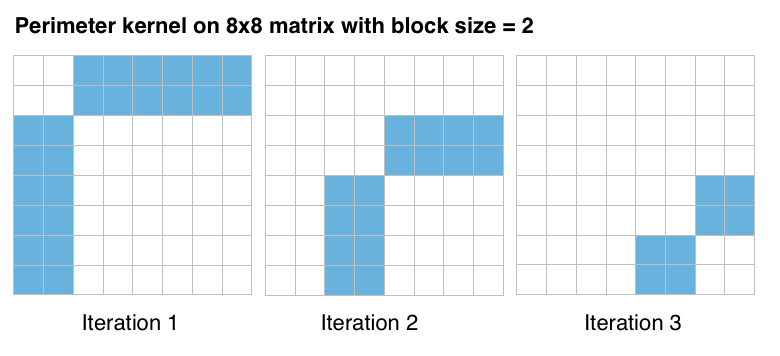
\includegraphics[width=0.6\textwidth]{figures/PerimeterKernel2.png}
    \caption{Perimeter \emph{kernel} algorithm on 8x8 matrix with block size = 2.}
    \label{PerimeterKernel2}
\end{figure}

\par{This \emph{kernel}, like the other two \emph{kernels}, is enqueued multiple times by 
    the host, each time to operate on a different portion of the matrix, 
    as shown above.}

\par{At each iteration of the loop in the host code, the total number of 
    \emph{work groups} is decreased by one. Eventually, in the last iteration of 
    the loop, only one \emph{work group} will be enqueued. Since \emph{work groups} are 
    scheduled in parallel on the Xeon Phi and Xeon CPU, this means that the 
    parallelism of the algorithm reduces as the computation proceeds. 
    There is guaranteed to be at least some under-utilisation of the hardware 
    threads due to the decreasing number of \emph{work groups}.}

\par{The opposite is true for the GPU. The number of \emph{work items} per 
    \emph{work group} increases for greater block sizes. This increases the 
    parallelism of the algorithm on the GPU. Table \ref{tab:lu2} summarises some 
    of the relevant parameters.}

\begin{table}[!h]
    \centering
    \begin{tabular}{| c | c | c | c |}
    \hline
    \emph{Block Size} & \emph{Data Size / Work Group} & 
    \emph{Starting Number of Work Groups} & 
    \emph{\#Work-Items / Work-Group} \\ \hline
    2 & 2x2 & 2047 & 4 \\ \hline
    4 & 4x4 & 1023 & 8 \\ \hline
    8 & 8x8 & 511 & 16 \\ \hline
    16 & 16x16 & 255 & 32 \\ \hline
    32 & 32x32 & 127 & 64 \\ \hline
    64 & 64x64 & 63 & 128 \\ \hline
    \end{tabular}
    \caption{Perimeter \emph{kernel} summary.}
    \label{tab:lu2}
\end{table}

\par{The performance of this \emph{kernel} can be explained as a compromise between 
    a number of factors. Firstly, a greater block size will decrease the 
    number of \emph{work groups} and increase the number of \emph{work items} per \emph{work group}. 
    For example, with a block size of 32, there will be a maximum of 127 work 
    groups, reducing to 1 \emph{work group} as the computation proceeds, but there 
    will be 64 \emph{work items} per \emph{work group}. In this case, the algorithm would 
    be under-utilising the hardware threads of the Xeon CPU and the Xeon Phi 
    with a small number of \emph{work groups}, but making use of the parallelism 
    available in the GPU with a larger number of \emph{work items} per \emph{work group}.}

\par{A greater block size reduces the overhead of loading data from global to 
    local memory, since more data is loaded to local memory at each execution. 
    For each greater block size, the total number of floating-point operations 
    also approximately doubles.}

\begin{figure}[!h]
    \centering
    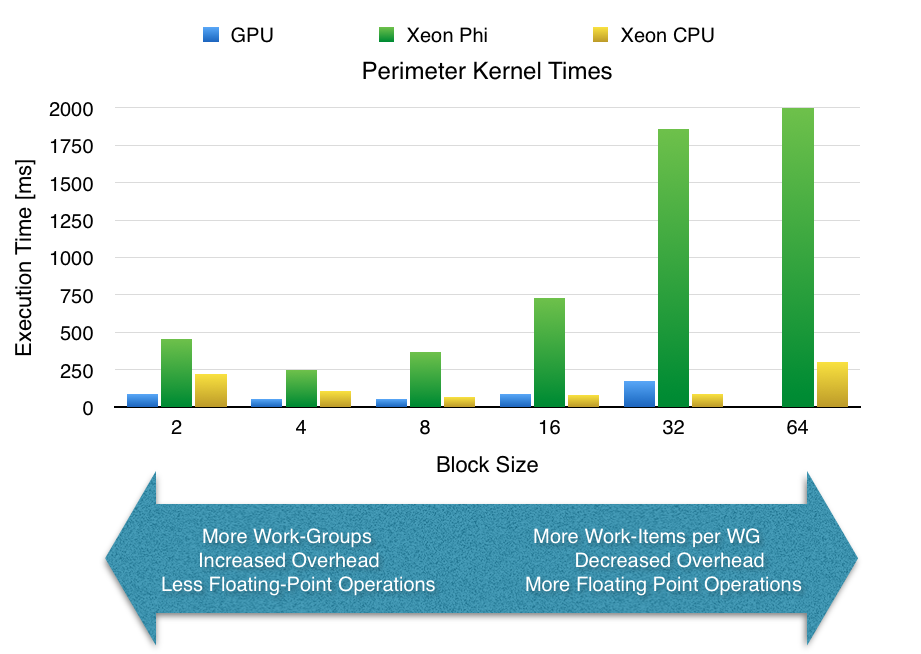
\includegraphics[width=0.6\textwidth]{figures/PerimeterKernel1.png}
    \caption{4096x4096 perimeter \emph{kernel} times.}
    \label{PerimeterKernel1}
\end{figure}

\par{Figure \ref{PerimeterKernel1} summarises these points. An increase in block size 
    effectively reduces the parallelism of the algorithm on the Xeon CPU 
    and Xeon Phi, but reduces the overhead incurred from high-latency data 
    transfers. For the GPU, the increase in block size gives rise to a higher
    level of parallelism, since \emph{work items} are scheduled in parallel on the 
    cores within each streaming multiprocessor. Unfortunately, the fact that 
    the total number of floating point operations increases according to the 
    block size skews the results.}

